\section{Programslut}
\label{sec:programslut}

När körningen avslutas visas statistik från körningen på den inkopplade
touchdisplayen. Användaren kan välja om hen vill se den genomsnittliga varvtiden
för vardera bil eller den genomsnittliga varvtiden för båda bilarna samtidigt.

\subsection{Varvtider}

Användaren kan välja att se varvtider från körningen som avslutades. Displayen
visar dels en tabell med referenstid, genomsnittlig varvtid och
standardavvikelse och dels en graf över alla varvtider för den ena av bilarna.
Grafen är en vanlig ''scatter plot'' med linjer mellan punkterna. Utritat finns
också den valda referenstiden och två linjer vid referenstiden $+$ 0,5~sekunder
respektive referenstiden $-$ 0,5~sekunder; den maximalt tillåtna avvikelsen från
referenstiden. Om två bilar körts kan användaren byta bil genom att trycka på en
knapp på displayen.

\subsection{Segmentstider}

Användaren kan också välja att se de genomsnittliga segmentstiderna från
körningen. Segmentstiderna ritas upp som stapeldiagram med en stapel per bil och
segment. Om två bilar körts visas istället två smalare staplar per segment.

\begin{figure}
	\centering
	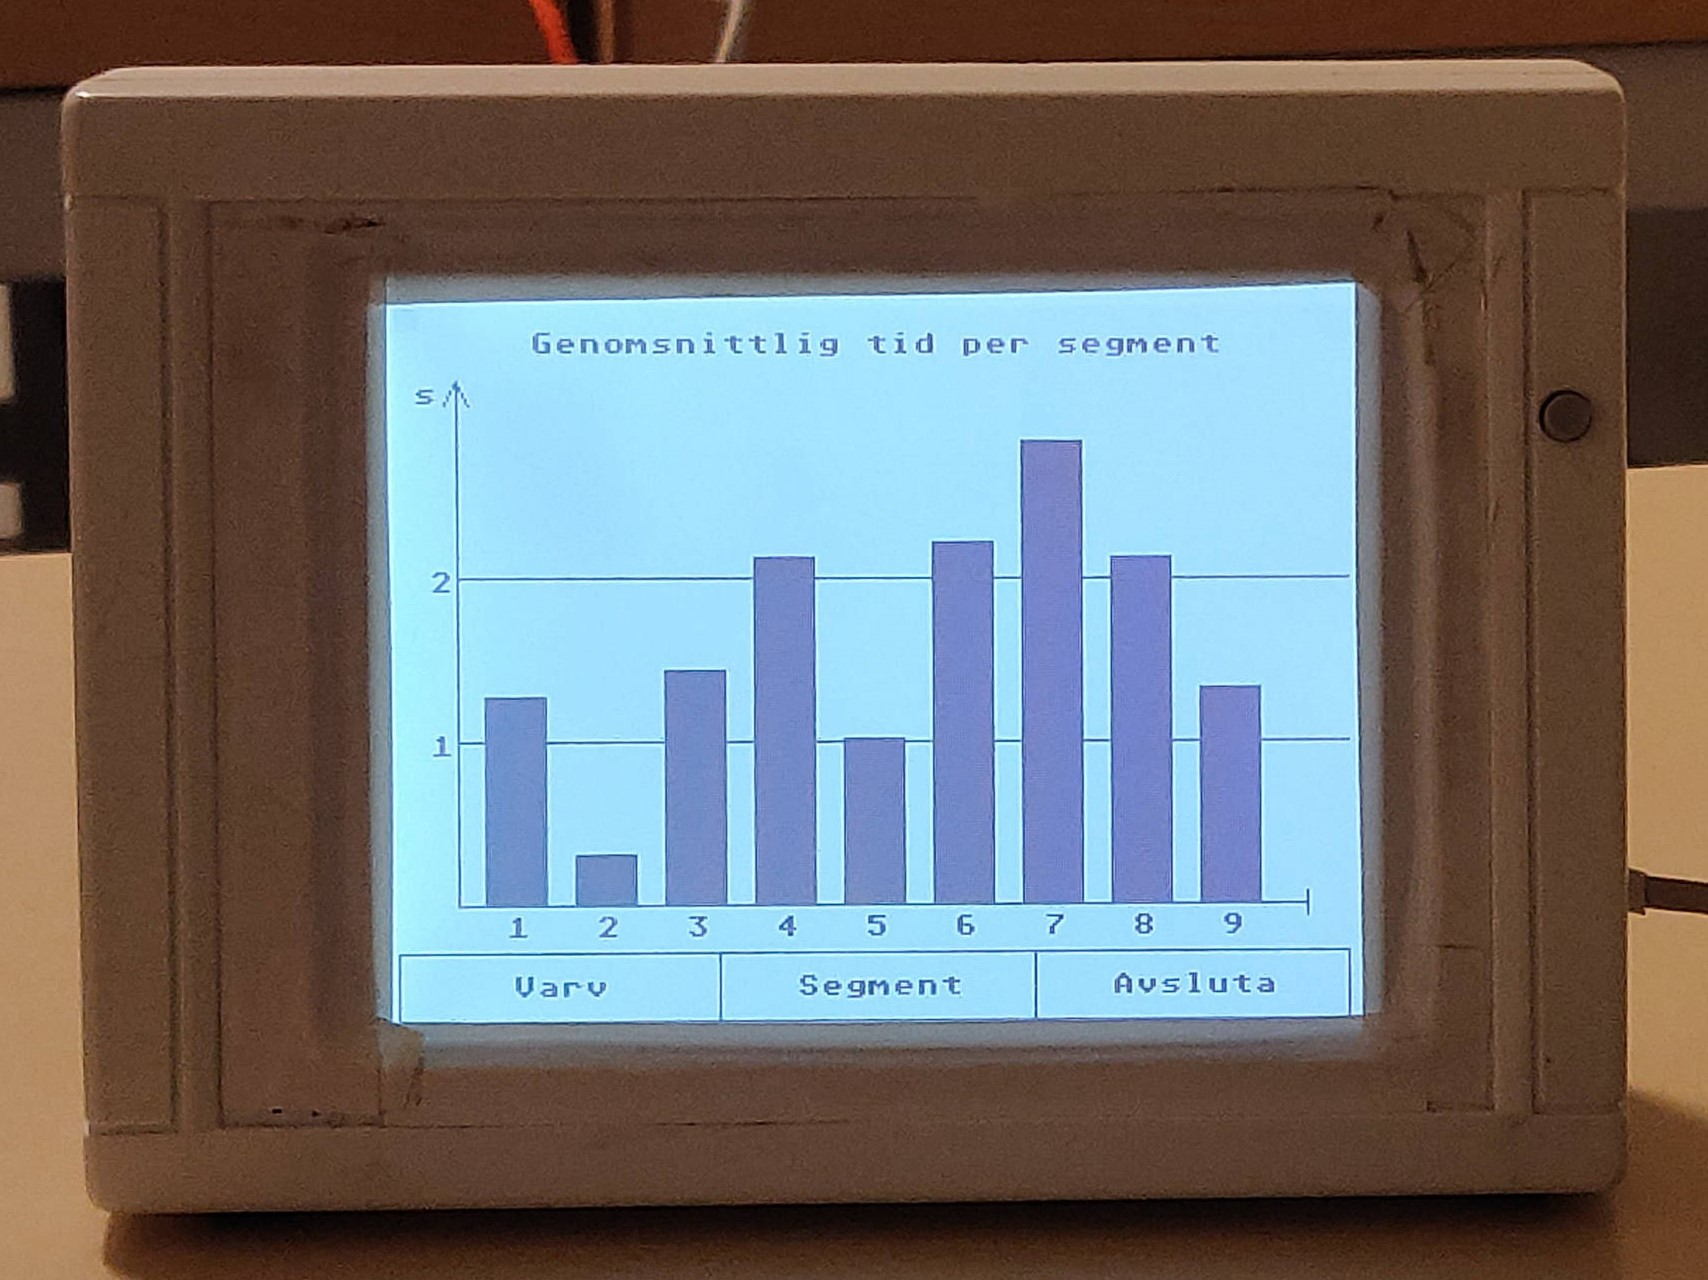
\includegraphics[width=0.75\linewidth] {Figures/genomsnitt_segment}
	\caption{Genomsnittliga segmentstider som de visas på displayen.}
	\label{fig:display-seg}
	
	\vspace*{2\floatsep}% https://tex.stackexchange.com/q/26521/5764
	
	\centering
	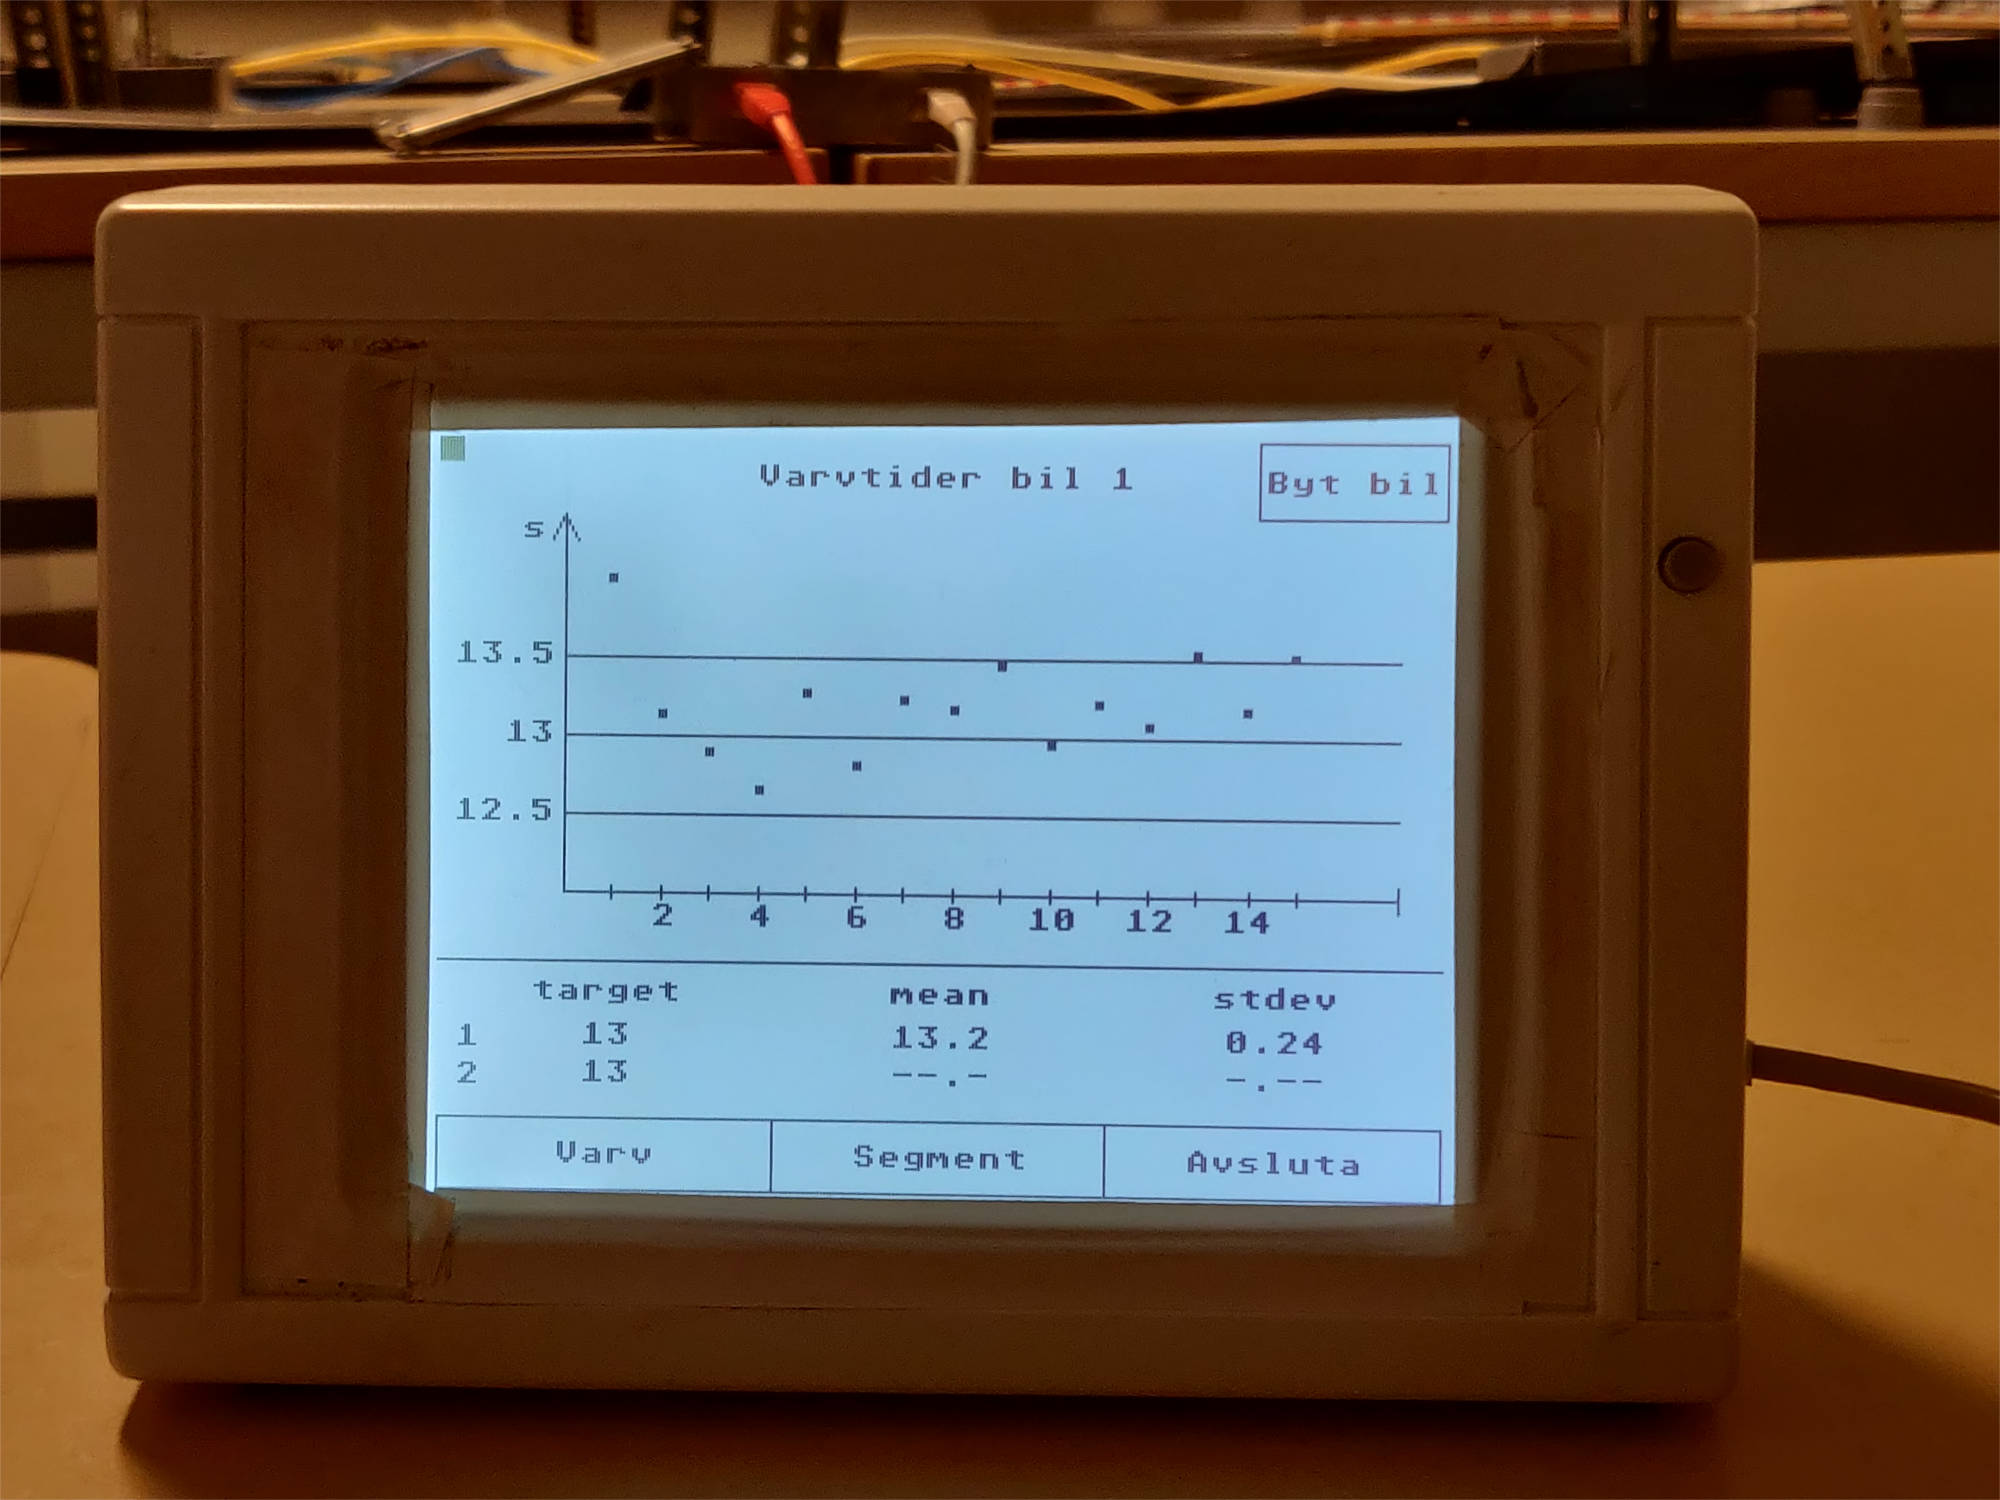
\includegraphics [width=0.75\linewidth] {Figures/varvtider}
	\caption{Varvtider som de visas på displayen.}
	\label{fig:display-lap}
\end{figure}
